\documentclass[10pt]{article}
\usepackage[margin=1in]{geometry}
\usepackage{libertine}
\usepackage[scaled=0.92]{helvet}
\usepackage{newtxmath}
\usepackage[T1]{fontenc}
\usepackage{microtype}
\usepackage{booktabs}
\usepackage{tikz}
\usetikzlibrary{positioning}
\usepackage{xcolor}
\usepackage{fancyhdr}
\usepackage{enumitem}
\usepackage{graphicx}
\usepackage{tabularx}
\usepackage{titlesec}

% ==== palette ====
\definecolor{slate}{HTML}{243B53}
\definecolor{petrol}{HTML}{1F5673}
\definecolor{accent}{HTML}{B5482F}
\definecolor{amber}{HTML}{C9852B}
\definecolor{teal}{HTML}{2A7F7F}
\definecolor{softgrey}{HTML}{EEF1F4}
\definecolor{midgrey}{HTML}{8A97A5}
\definecolor{green}{HTML}{4E7A55}

\renewcommand{\familydefault}{\rmdefault}
\titleformat{\section}{\sffamily\large\bfseries\color{slate}}{\thesection.}{0.5em}{}
\titleformat{\subsection}{\sffamily\normalsize\bfseries\color{petrol}}{\thesubsection}{0.5em}{}
\setlist[description]{font=\sffamily\bfseries\color{petrol},leftmargin=6.2em,style=sameline}

\pagestyle{fancy}\fancyhf{}
\renewcommand{\headrulewidth}{0pt}
\fancyfoot[L]{\footnotesize\sffamily\color{midgrey}AI Analytics, contact@aianalytics.tech}
\fancyfoot[R]{\footnotesize\sffamily\color{midgrey}\thepage}

% ==== risk pill ====
\newcommand{\pill}[2]{\tikz[baseline=-0.6ex]\node[fill=#1,text=white,font=\sffamily\bfseries\footnotesize,inner xsep=6pt,inner ysep=2.5pt,rounded corners=2pt]{#2};}
\newcommand{\pcrit}{\pill{accent}{CRITICAL}}
\newcommand{\phigh}{\pill{amber}{HIGH}}
\newcommand{\pelev}{\pill{teal}{ELEVATED}}
\newcommand{\pmed}{\pill{petrol}{MEDIUM}}

% ==== risk card ====
\newcommand{\riskcard}[3]{%
  \par\vspace{4pt}\noindent\colorbox{softgrey}{\parbox{\dimexpr\textwidth-2\fboxsep}{%
  \sffamily\bfseries\color{slate}#1\quad #2\hfill #3}}\par\vspace{1pt}}

\begin{document}

% ================= MASTHEAD =================
\thispagestyle{fancy}
\noindent{\sffamily\bfseries\Large\color{slate}AI\,Analytics}\hfill{\sffamily\footnotesize\color{midgrey}contact@aianalytics.tech}\\[-2pt]
\textcolor{slate}{\rule{\textwidth}{1.2pt}}\\[2pt]
{\sffamily\footnotesize\color{petrol}COUNTRY AND PROGRAM RISK ANALYSIS}\\[6pt]
{\sffamily\bfseries\LARGE\color{slate}Bolivia: risk to the IMF Extended Fund Facility}\\[3pt]
{\sffamily\large\color{petrol}Can the program deliver its objectives over 36 months and just after?}\\[6pt]
{\sffamily\footnotesize Version 1\quad\textbar\quad Prepared by AI Analytics\quad\textbar\quad September 2026}\\[2pt]
{\sffamily\scriptsize\color{midgrey}Analytical risk assessment; not investment or legal advice. Quantitative backbone: the Augmented MFMOD-Bolivia debt-sustainability analysis (AI Analytics).}
\vspace{8pt}

% ================= AT A GLANCE =================
\noindent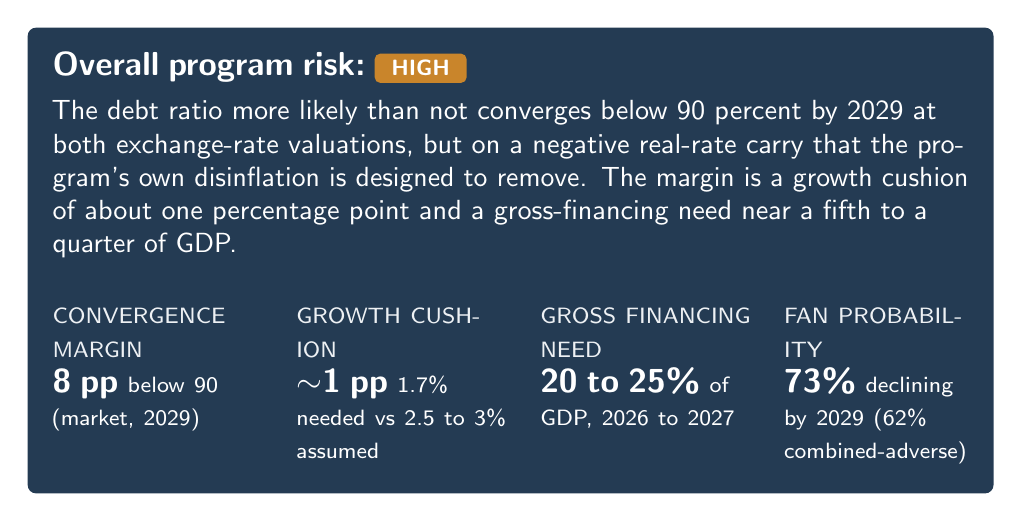
\begin{tikzpicture}
\node[fill=slate,text=white,rounded corners=3pt,inner sep=9pt,text width=\dimexpr\textwidth-2\fboxsep-8pt]{%
\sffamily
{\bfseries\large Overall program risk:}\ \pill{amber}{HIGH}\\[4pt]
{\normalsize The debt ratio more likely than not converges below 90 percent by 2029 at both exchange-rate valuations, but on a negative real-rate carry that the program's own disinflation is designed to remove. The margin is a growth cushion of about one percentage point and a gross-financing need near a fifth to a quarter of GDP.}\\[6pt]
\begin{tabular}{@{}p{0.23\textwidth}p{0.23\textwidth}p{0.23\textwidth}p{0.22\textwidth}@{}}
{\footnotesize\color{softgrey}CONVERGENCE MARGIN} & {\footnotesize\color{softgrey}GROWTH CUSHION} & {\footnotesize\color{softgrey}GROSS FINANCING NEED} & {\footnotesize\color{softgrey}FAN PROBABILITY}\\[1pt]
{\bfseries\large 8 pp}\ {\footnotesize below 90 (market, 2029)} & {\bfseries\large $\sim$1 pp}\ {\footnotesize 1.7\% needed vs 2.5 to 3\% assumed} & {\bfseries\large 20 to 25\%}\ {\footnotesize of GDP, 2026 to 2027} & {\bfseries\large 73\%}\ {\footnotesize declining by 2029 (62\% combined-adverse)}\\
\end{tabular}};
\end{tikzpicture}

% ================= EXECUTIVE SUMMARY =================
\section{Executive summary}
On the program's own assumptions the public-debt ratio is sustainable. Sector Publico No Financiero
(SPNF) debt falls from 80 percent of GDP at the official valuation and about 90 percent at the market
valuation at end-2025, to about 81 and 82 percent by 2029, meeting the program's stated below-90-percent
trajectory at both valuations. The result is not carried by the fiscal effort. It is carried by a
negative gap between the effective real interest rate and real growth, the historical norm for an
economy with concessional external debt and a repressed domestic market. The primary adjustment of
about 8.5 percent of GDP over 2026 to 2029 stops the deficit from adding to the stock; the decline
comes from the carry.

Two risks are linked into the program's critical failure mode.

\pcrit\ \textbf{Growth (R1).} The convergence depends on a recovery to about 2.5 to 3 percent by 2029,
and the minimum sustained growth that holds the market-rate ratio below 90 percent by 2029 is 1.7
percent, a cushion of about one point. Two independent instruments, a structural model at minus 3.3
percent for 2025 and a combustion nowcast at minus 2.8 percent for the September 2025 to August 2026
window, read the near-term contraction deeper than the program's minus 1.6, so the program is the
optimistic outlier on the part that can be checked, and the recovery is the part that cannot.

\phigh\ \textbf{The success trap (R4).} The program targets single-digit inflation by 2028, and the
effective rate reprices upward as the concessional stock rolls off at the 20-to-25-percent-of-GDP
financing need. Program success turns the gap between the real rate and growth positive around 2030;
the ratio then stops falling and climbs toward the 90 line again, and a primary surplus of about 1
percent of GDP becomes the condition for renewed decline.

The link is that the disinflation which the program needs is the same force that removes the carry now
doing the deleveraging. The base case holds because the two do not bind at once in the central path;
the risk is the joint state of a growth shortfall and a repricing success, together with a
capital-heavy consolidation and a contingent-liability crystallization that on its central estimate
breaches 90 on its own.

% ================= RISK DASHBOARD =================
\section{Risk dashboard}
\begin{minipage}[t]{0.52\textwidth}
\vspace{0pt}
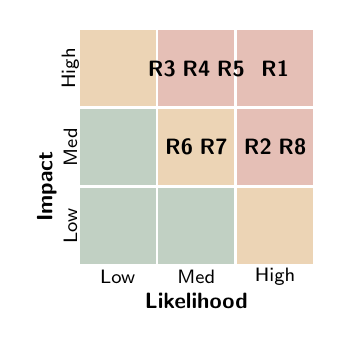
\begin{tikzpicture}[scale=1.0,every node/.style={font=\sffamily\footnotesize}]
% cells: x=likelihood (1 low..3 high), y=impact (1..3)
\foreach \x/\y/\c in {1/1/green,2/1/green,3/1/amber,1/2/green,2/2/amber,3/2/accent,1/3/amber,2/3/accent,3/3/accent}{
  \fill[\c!35] (\x,\y) rectangle (\x+1,\y+1);
  \draw[white,line width=1pt] (\x,\y) rectangle (\x+1,\y+1);}
% risk codes
\node at (3.5,3.5){\bfseries R1};
\node at (3.5,2.5){\bfseries R2\;R8};
\node at (2.5,3.5){\bfseries R3\;R4\;R5};
\node at (2.5,2.5){\bfseries R6\;R7};
\node[rotate=90] at (0.6,2){\bfseries Impact};
\node at (2.5,0.55){\bfseries Likelihood};
\foreach \x/\l in {1.5/Low,2.5/Med,3.5/High}{\node at (\x,0.85){\scriptsize\l};}
\foreach \y/\l in {1.5/Low,2.5/Med,3.5/High}{\node[rotate=90] at (0.9,\y){\scriptsize\l};}
\end{tikzpicture}
\end{minipage}\hfill
\begin{minipage}[t]{0.44\textwidth}
\vspace{2pt}\sffamily\footnotesize
\textbf{\color{slate}Legend}\\[3pt]
\pcrit\ R1 Growth shortfall and recovery optimism\\[2pt]
\phigh\ R2 Fuel cost-recovery social and price shock\\[2pt]
\phigh\ R3 Debt-stock and gross-financing pressure\\[2pt]
\phigh\ R4 Disinflation-repricing success trap\\[2pt]
\phigh\ R5 Contingent-liability crystallization\\[2pt]
\pelev\ R6 External and terms-of-trade downside\\[2pt]
\pelev\ R7 Financial-sector fragility\\[2pt]
\phigh\ R8 Reform ownership and compensation timing\\
\end{minipage}

% ================= RISK REGISTER =================
\section{Risk register}
\riskcard{R1}{Growth shortfall and recovery optimism}{\pcrit}
\begin{description}
\item[Channel] The debt path converges only if growth recovers to about 2.5 to 3 percent by 2029; below the 1.7-percent threshold the market-rate ratio stays above 90 in 2029.
\item[Evidence] Bifurcation frontier in the DSA; the independent growth cross-check (model minus 3.3, nowcast minus 2.8, both deeper than the program's minus 1.6); scenario S9 shifts the 2029 ratio to 82/84 and cuts the cushion to about 6 points.
\item[Likelihood] High. \item[Impact] High.
\item[Watch] SPNF primary balance floor (Cuadro 1); the combustion nowcast refresh; the official activity index at the five-to-six-month lead.
\item[Mitigant] Protect the investment share of the consolidation; a medium-term independent growth read to test the recovery assumption.
\end{description}

\riskcard{R2}{Fuel cost-recovery social and price shock}{\phigh}
\begin{description}
\item[Channel] The January-2027 move to cost-recovery pricing (DS 5652) and the large-consumer diesel differential (Bs 18 versus Bs 9.80, DS 5676) raise transport and food prices and carry social-unrest risk.
\item[Evidence] MEFP risk section (p.4, para 9); the program's own delay of the subsidy removal to 2027; scenario S3, where a half-delivered saving and 0.5 point of lost growth raise the 2029 ratio to 83/85.
\item[Likelihood] High. \item[Impact] Medium to High.
\item[Watch] The 2027 budget with no Treasury or state-enterprise fuel subsidy (structural benchmark, end-December 2026); the social-assistance floor (Cuadro 1).
\item[Mitigant] Compensation that leads rather than lags the price step; targeted transfers through the social registry.
\end{description}

\riskcard{R3}{Debt-stock and gross-financing pressure}{\phigh}
\begin{description}
\item[Channel] Gross financing needs run at 20 to 25 percent of GDP; the foreign-currency third of the stock revalues with the exchange rate; external disbursements and Congress approvals gate the roll.
\item[Evidence] DSA gross-financing table; the mechanical 2026 rise on the official-rate unification; the market valuation near 90 and the full-parallel valuation on the order of 100 to 105 percent at end-2025.
\item[Likelihood] Medium to High. \item[Impact] High.
\item[Watch] Net international reserve floors and no-external-arrears criterion (Cuadro 1); the external-to-local liability swap execution.
\item[Mitigant] The IMF and multilateral disbursements; the reserve accumulation floors; the liability-management operation.
\end{description}

\riskcard{R4}{Disinflation-repricing success trap}{\phigh}
\begin{description}
\item[Channel] As inflation falls to single digits and the effective rate reprices upward, the gap between the real rate and growth turns positive and the programmed zero primary no longer holds the ratio down.
\item[Evidence] Scenario S10: the gap turns positive around 2030, the ratio stops falling and rises to about 88/90 by 2031 and 94/96 by 2035, and the stabilizing primary becomes a surplus of about 0.95 percent of GDP.
\item[Likelihood] Medium (conditional on program success). \item[Impact] High.
\item[Watch] The base-money ceiling and inflation path (Cuadro 1, p.10); the marginal rate on new external and local issuance.
\item[Mitigant] A medium-term fiscal framework that plans the transition from zero primary to a small surplus before the carry reverses.
\end{description}

\riskcard{R5}{Contingent-liability crystallization}{\phigh}
\begin{description}
\item[Channel] State-enterprise losses, fuel-trader arrears, the central-bank credit programs, and the pension-fund exposure to the public sector can move onto the debt stock as a stock-flow adjustment.
\item[Evidence] Right-sized S6: a central bundle of about 7 percent of GDP (fuel-trader arrears about 2 percent, residual arrears about 0.9 percent, state-enterprise losses and the credit-program wind-down the rest) puts the 2028 ratio at 90/92, breaching 90 at both valuations; the range runs 4 to 12 percent.
\item[Likelihood] Medium. \item[Impact] High.
\item[Watch] The arrears audit and state-enterprise restructuring (MEFP p.6 to 7); the fiscal-risk publication (structural benchmark, end-June 2027).
\item[Mitigant] The arrears clearance strategy; state-enterprise reform; publication of the full public-sector liability perimeter.
\end{description}

\riskcard{R6}{External and terms-of-trade downside}{\pelev}
\begin{description}
\item[Channel] The current account is assumed to move to surplus in 2026 to 2027; a terms-of-trade reversal or higher energy import prices, together with disbursement timing, reopen the external gap.
\item[Evidence] MEFP risk section (p.4, para 9); scenario S4, where a 150-basis-point rise in the external rate and a disbursement slip hold the ratio near 87/89 with little decline.
\item[Likelihood] Medium. \item[Impact] Medium to High.
\item[Watch] Reserve floors; the current-account path; the timing of multilateral and bilateral disbursements.
\item[Mitigant] The reserve accumulation floors; the multilateral financing commitments (about 70 percent of external debt multilateral).
\end{description}

\riskcard{R7}{Financial-sector fragility}{\pelev}
\begin{description}
\item[Channel] Foreign-currency deposits, the central-bank credit-program unwind, the pension-fund exposure, and asset quality under higher rates are transmission points during the transition to market-based policy.
\item[Evidence] MEFP risk section and the financial-stability commitments (p.4 para 9; p.12 to 13, para 29 to 32).
\item[Likelihood] Medium. \item[Impact] High.
\item[Watch] The solvency and liquidity stress tests (structural benchmark, end-March 2027); the credit-program repayment plan; deposit dynamics.
\item[Mitigant] The stress-testing and resolution-regime program; the deposit-return schedule; the deposit-insurance unit.
\end{description}

\riskcard{R8}{Reform ownership and compensation timing}{\phigh}
\begin{description}
\item[Channel] Whether compensation leads or lags the January-2027 fuel step, and whether the reform holds a social coalition, decides if the primary path survives contact with the political cycle.
\item[Evidence] The political-economy analysis of rent and reform ownership; the program's own reliance on sustained social consent (MEFP p.1, para 2); scenario S3 and S7.
\item[Likelihood] High. \item[Impact] Medium to High.
\item[Watch] The social-assistance floor delivery (Cuadro 1); the social registry and means-testing framework (structural benchmark, end-March 2027).
\item[Mitigant] A resource-dividend or universal-transfer design that makes the citizenry a residual claimant; compensation sequenced ahead of the price step.
\end{description}

% ================= SCENARIO ANALYSIS =================
\section{Scenario analysis}
The debt paths are reduced-form, reported at the official and the market valuation. Scenarios are
illustrative structured stresses, not forecasts. S0 is the program baseline; S1 to S8 are the DSA
stresses; S9 and S10 are the new independent-growth and success-case scenarios.

\begin{table}[h]\centering\footnotesize
\caption{SPNF debt, percent of GDP, official / market valuation}
\begin{tabular}{lccccc}
\toprule
Scenario & 2027 & 2028 & 2029 & 2031 & 2035\\
\midrule
S0 baseline & 85/87 & 83/85 & 81/82 & 77/78 & 71/72\\
S1 growth shortfall & 87/89 & 85/87 & 83/85 & 79/81 & 73/75\\
S4 external downside & 89/91 & 88/90 & 87/89 & 85/87 & 83/85\\
S6 contingent liabilities (7\%) & 89/91 & 90/92 & 87/89 & 83/85 & 76/78\\
S7 combined adverse & 88/90 & 88/90 & 87/89 & 84/86 & 77/79\\
S8 growth-protective & 85/87 & 83/85 & 80/81 & 75/77 & 69/70\\
\textbf{S9 ISAE near-term (central)} & 87/89 & 84/86 & 82/84 & 78/80 & 72/73\\
\textbf{S10 disinflation-repricing} & 86/88 & 86/88 & 86/88 & 88/90 & 94/96\\
\bottomrule
\end{tabular}
\end{table}

\begin{figure}[h]\centering
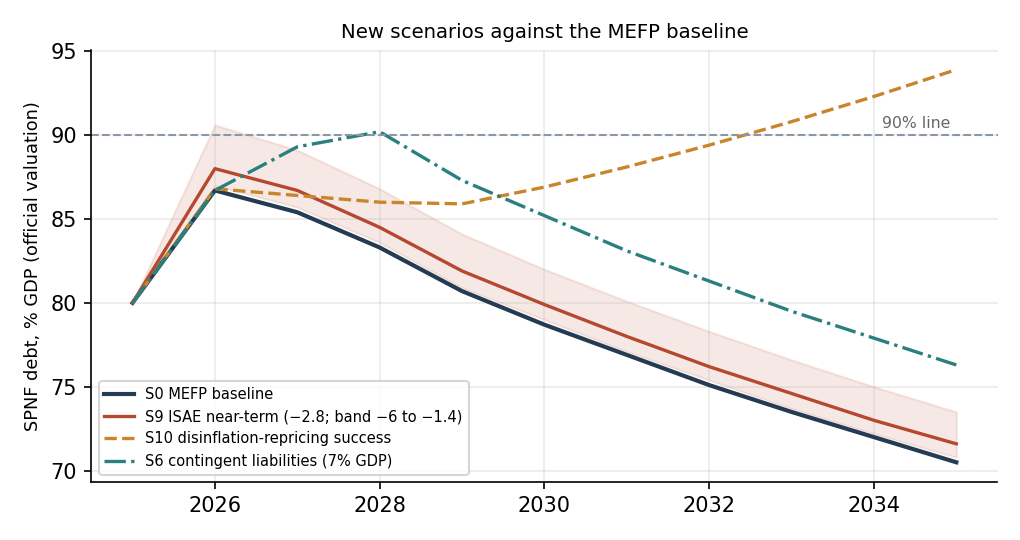
\includegraphics[width=0.82\textwidth]{../exhibits/fig_scenarios.png}
\caption{New scenarios against the baseline. The success case (S10) is the only path that turns back up.}
\end{figure}

\begin{figure}[h]\centering
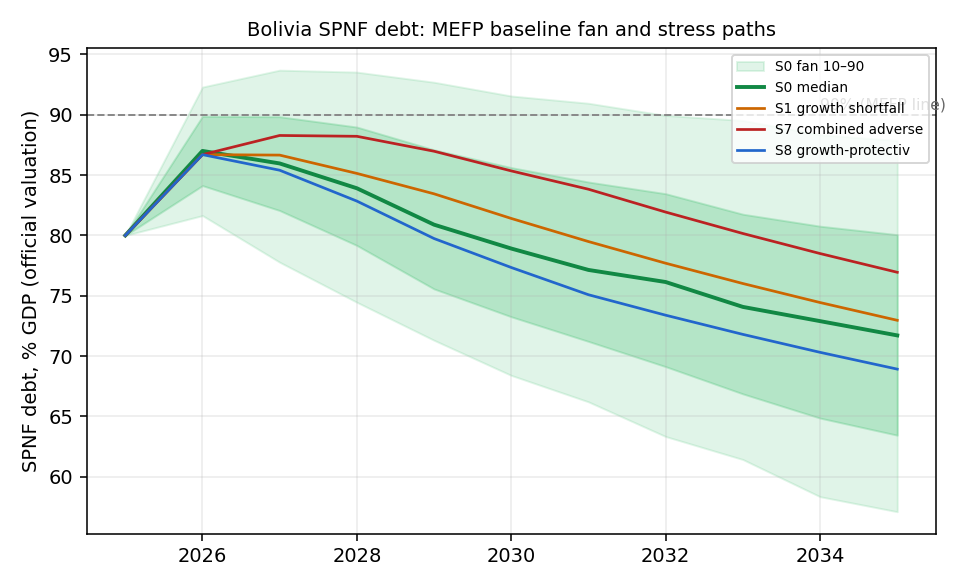
\includegraphics[width=0.82\textwidth]{../exhibits/fig_debt_fan.png}
\caption{Baseline stochastic fan (1{,}000 draws, seed 20260910) with the growth-shortfall, combined-adverse, and growth-protective paths.}
\end{figure}

\textbf{The bifurcation.} On the program's assumptions the ratio converges. It stalls above 90 and a
primary surplus becomes the condition for decline under one combination: a deeper near-term
contraction (S9), the disinflation and repricing that turn the carry positive (S10), and a
capital-heavy consolidation that lowers potential growth (the gap between S2 and S8). Each element
alone is survivable; the combination is the program's critical scenario.

% ================= GROWTH CROSS-CHECK =================
\section{Independent growth cross-check}
\begin{figure}[h]\centering
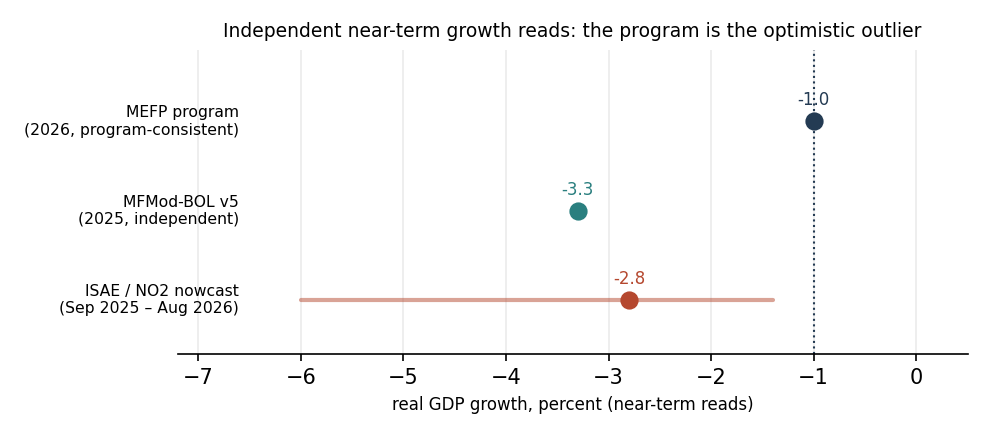
\includegraphics[width=0.80\textwidth]{../exhibits/fig_growth_crosscheck.png}
\caption{Three independent near-term growth reads. The combustion nowcast carries its bracket.}
\end{figure}
Two of the three independent instruments put the 2025 to 2026 contraction materially deeper than the
program, so the program's near-term growth is the optimistic outlier, and the same optimism is the
natural prior on its recovery assumption. The nowcast bracket, not its point, is carried into the S9
debt path. The nowcast is not extended past its horizon; the 2028-and-after path stays program-based
and is flagged as such.

% ================= MONITORING DASHBOARD =================
\section{Monitoring dashboard}
Each risk is mapped to a quantitative criterion or structural benchmark and to the review calendar.
The first review is scheduled for December 2026 on the end-September 2026 criteria.

\begin{table}[h]\centering\footnotesize
\begin{tabularx}{\textwidth}{llX}
\toprule
Risk & Quantitative anchor & Trigger to watch\\
\midrule
R1 & SPNF primary floor (Cuadro 1) & primary miss; nowcast refresh below the program near-term path\\
R2 & 2027 budget, no fuel subsidy (SB, end-Dec 2026) & delay or partial reversal of the January-2027 step\\
R3 & NIR floors; no external arrears (Cuadro 1) & disbursement slip; reserve floor miss; arrears accumulation\\
R4 & base-money ceiling; inflation path & inflation reaching single digits with the rate repricing up\\
R5 & fiscal-risk publication (SB, end-Jun 2027) & a contingent liability moving onto the stock above about 4 to 5 percent of GDP\\
R6 & NIR floors; current account & terms-of-trade reversal; external-rate rise\\
R7 & solvency and liquidity stress tests (SB, end-Mar 2027) & asset-quality deterioration; deposit outflow\\
R8 & social-assistance floor (Cuadro 1) & compensation lagging the fuel step; social-registry delay\\
\bottomrule
\end{tabularx}
\end{table}

% ================= OUTLOOK =================
\section{Outlook}
The base case is convergence below 90 percent by 2029 at both exchange-rate valuations, on a negative
carry, more likely than not on the fan. Three swing factors decide whether it holds.
\begin{itemize}[leftmargin=1.4em,itemsep=1pt]
\item \textbf{Post-2028 growth.} The recovery to about 2.5 to 3 percent is the load-bearing
assumption and the least independently verifiable one; the cushion to the 1.7-percent threshold is
about one point.
\item \textbf{The composition of the consolidation.} Cutting current spending rather than capital is
worth about 2 to 4 points of the debt ratio by 2035, the difference between the growth-protective and
investment-compression paths.
\item \textbf{Whether compensation leads or lags the January-2027 fuel step.} The sequencing decides
the social consent on which the primary path depends.
\end{itemize}
The program can deliver its objectives, and on the central path it does. The risk is concentrated, not
diffuse: it sits in the joint state where the program succeeds at disinflation, growth disappoints,
and a public-sector liability crystallizes, and it is in that state that the zero primary target
becomes insufficient and a surplus becomes the condition for a falling ratio.

\newpage
% ================= APPENDIX =================
\section*{Appendix A: debt paths, both valuations}
\begin{table}[h]\centering\footnotesize
\caption{SPNF debt, percent of GDP, official / market valuation, all scenarios}
\begin{tabular}{lcccccccc}
\toprule
Scenario & 2026 & 2027 & 2028 & 2029 & 2030 & 2031 & 2033 & 2035\\
\midrule
S0 baseline & 87/89 & 85/87 & 83/85 & 81/82 & 79/80 & 77/78 & 73/75 & 71/72\\
S1 growth shortfall & 87/89 & 87/89 & 85/87 & 83/85 & 81/83 & 79/81 & 76/78 & 73/75\\
S2 investment compression & 87/89 & 85/87 & 84/86 & 82/83 & 80/82 & 79/80 & 75/77 & 72/74\\
S3 reform reversal & 87/89 & 87/89 & 86/88 & 83/85 & 81/83 & 79/81 & 76/77 & 73/74\\
S4 external downside & 89/91 & 89/91 & 88/90 & 87/89 & 86/88 & 85/87 & 84/86 & 83/85\\
S5 second FX adjustment & 87/89 & 87/88 & 83/85 & 80/82 & 78/80 & 76/78 & 73/75 & 70/72\\
S6 contingent liab. (7\%) & 87/89 & 89/91 & 91/92 & 88/89 & 86/87 & 84/85 & 80/81 & 77/78\\
S7 combined adverse & 87/89 & 88/90 & 88/90 & 87/89 & 85/87 & 84/86 & 80/82 & 77/79\\
S8 growth-protective & 87/89 & 85/87 & 83/85 & 80/81 & 77/79 & 75/77 & 72/73 & 69/70\\
S9 ISAE near-term & 88/90 & 87/89 & 84/86 & 82/84 & 80/82 & 78/80 & 75/76 & 72/73\\
S10 disinflation-repricing & 87/89 & 86/88 & 86/88 & 86/88 & 87/89 & 88/90 & 91/93 & 94/96\\
\bottomrule
\end{tabular}
\end{table}

\section*{Appendix B: identification and provenance}
\textbf{Status of headlines.} Baseline anchors (2025 growth, primary floors, zero primary by 2029,
debt 80/90 at end-2025, the 90-by-2029 path) are program figures, page-cited in the debt-sustainability
analysis. The 2026-to-2035 growth and inflation glide is program-consistent, not a program figure. The
interest-rate path, the foreign-currency share, and the amortization profile are reduced-form
calibrations. All debt paths, the gap between the real rate and growth, the stabilizing values, and the
financing needs are reduced-form results of the debt-dynamics identity. Scenarios S1 to S10 are
illustrative structured stresses. The fan probabilities are inference around the identity with the
historical joint distribution of growth and the real rate.

\textbf{Reduced-form status.} The debt path is identity-based, not a full structural solve. The
Augmented MFMOD-Bolivia model supplies structure and elasticities and an independent growth read; its
own 2025 call is minus 3.3 percent, and it is not used as the baseline generator.

\textbf{Exchange-rate valuation.} Every debt and financing figure is reported at the official peg
valuation (6.96 Bs/USD) and the market valuation (a reference rate near 9.8 that reconciles the
program's 90-percent end-2025 figure). The full street-parallel valuation, near 13.5, is the adverse
bound and puts the end-2025 stock on the order of 100 to 105 percent. A single-rate figure is not a
result.

\textbf{GDP rebase.} The 2016/17 rebase breaks any ratio-to-GDP series; the spliced series is used for
the historical ratios and the fan distribution, and the unspliced series does not change the sign of
any headline.

\textbf{Frequency.} The data and the analysis are annual. No higher-frequency inference is drawn,
including from the within-year test points of Cuadro 1.

\textbf{Sources.} Program anchors: the Memorando de Politicas Economicas y Financieras. Historical
series: the fiscal database (SPNF 1990 to 2024, debt and GDP, INE consumer prices, the state-enterprise
directory). Near-term activity: the combustion nowcast (published reads). Model structure: the
Augmented MFMOD-Bolivia, AI Analytics.

\vspace{16pt}
\noindent\textcolor{slate}{\rule{\textwidth}{0.8pt}}\\[4pt]
{\sffamily\bfseries\color{slate}AI Analytics}\\[1pt]
{\sffamily\footnotesize Country and Program Risk Analysis, Version 1\quad\textbar\quad contact@aianalytics.tech}\\[1pt]
{\sffamily\scriptsize\color{midgrey}Analytical risk assessment; not investment or legal advice.}

\end{document}
